
\typeout{IJCAI--25 Instructions for Authors}


\documentclass{article}
\pdfpagewidth=8.5in
\pdfpageheight=11in

\usepackage{ijcai25}

\usepackage{amsmath}
\usepackage{amssymb}
\usepackage{mathtools}
\usepackage{amsthm}
\usepackage{enumitem}

\usepackage{times}
\usepackage{soul}
\usepackage{url}
\usepackage[hidelinks]{hyperref}
\usepackage[utf8]{inputenc}
\usepackage[small]{caption}
\usepackage{graphicx}
\usepackage{amsmath}
\usepackage{amsthm}
\usepackage{booktabs}
\usepackage{algorithm}
\usepackage{algorithmic}
\usepackage[switch]{lineno}

\usepackage{soul}
\usepackage{multirow}



\urlstyle{same}


\newtheorem{example}{Example}
\newtheorem{theorem}{Theorem}






\pdfinfo{
/TemplateVersion (IJCAI.2025.0)
}

\title{Electron Density-enhanced Molecular Geometry Learning}

\author{
    Author Name
    \affiliations
    Affiliation
    \emails
    email@example.com
}

\author{
Hongxin Xiang$^1$
\and
Jun Xia$^2$\and
Xin Jin$^3$\and
Wenjie Du$^4$\and
Li Zeng$^1$\And
Xiangxiang Zeng$^{1,}$\footnote{Corresponding author (xzeng@hnu.edu.cn)}\\
\affiliations
$^1$College of Computer Science and Electronic Engineering, Hunan University, Changsha, China\\
$^2$School of Engineering, Westlake University, Hangzhou, China\\
$^3$Eastern Institute of Technology, Ningbo, China\\
$^4$University of Science and Technology of China, Hefei, China\\
}

\begin{document}

\maketitle

\begin{abstract}


Electron density (ED), which describes the probability distribution of electrons in space, is crucial for accurately understanding the energy and force distribution in molecular force fields (MFF).
Existing machine learning force fields (MLFF) focus on mining appropriate physical quantities from the atom-level conformation to enhance the molecular geometry representation while ignoring the unique information from microscopic electrons.
In this work, we propose an efficient \textbf{E}lectronic \textbf{D}ensity representation framework to enhance molecular \textbf{G}eometric learning (called EDG), which leverages images rendered from ED to boost molecular geometric representations in MLFF.
Specifically, we construct a novel image-based ED representation, which consists of 2 million 6-view images with RGB-D channels, and design an ED representation learning model, called ImageED, to learn ED-related knowledge from these images. We further propose an efficient ED-aware teacher and introduce a cross-modal distillation strategy to transfer knowledge from the image-based teacher to the geometry-based students.
Extensive experiments on QM9 and rMD17 demonstrate that EDG can be directly integrated into existing geometry-based models and significantly improves the capabilities of these models (e.g., SchNet, EGNN, SphereNet, ViSNet) for geometry representation learning in MLFF with a maximum average performance increase of 33.7\%. Code and appendix are available at https://github.com/HongxinXiang/EDG

\end{abstract}

\section{Introduction}
\label{Introduction}


\begin{figure*}[htbp]
\centering
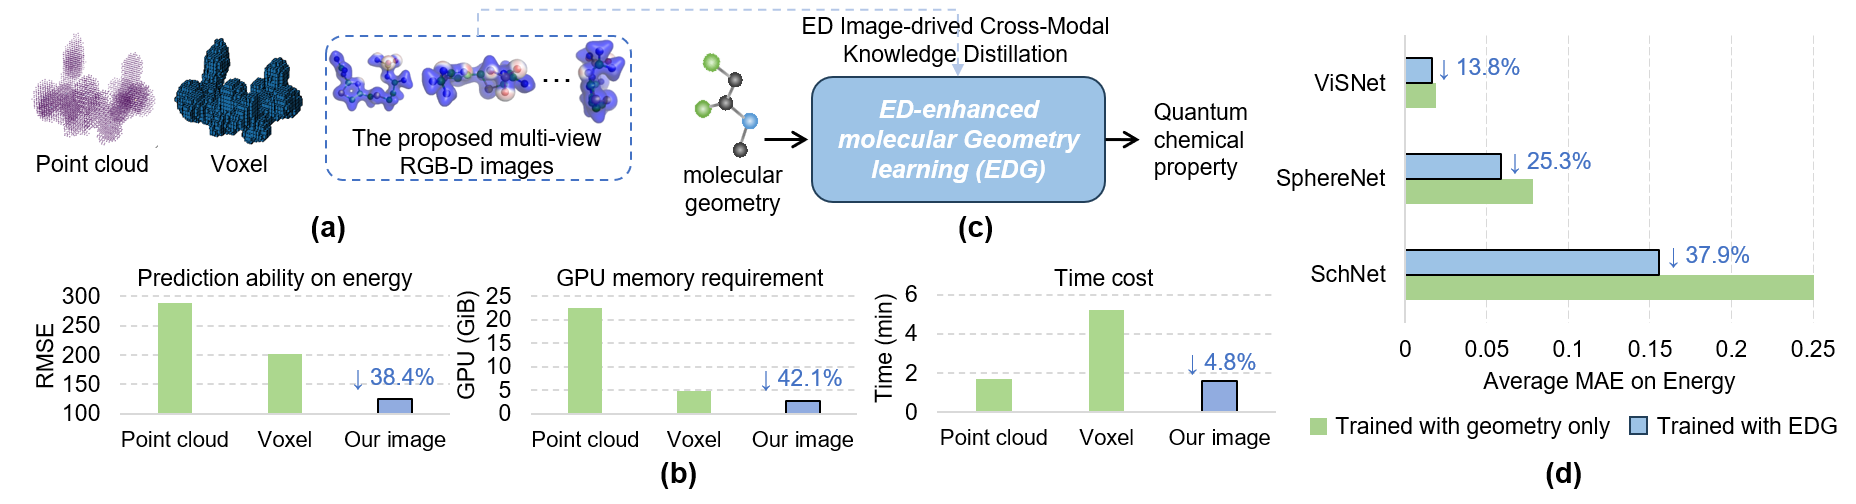
\includegraphics[width=16cm]{./imgs/introduction/Fig1_introduction.png}
\caption{(a) ED representation methods. (b) RMSE in energy prediction, GPU memory, and training time cost of different ED representations with the same experimental setting. (c) The proposed EDG framework, which uses multi-view ED images with RGB-D channels to enhance molecular geometry learning. (d) Average MAE performance on 10 energy prediction datasets of rMD17 by using or not using the EDG.}
\label{Fig1_Intro}
\vspace{-0.4cm}
\end{figure*}

Machine learning force fields (MLFF) is a computationally efficient and low-cost method for learning the interactions between atoms in molecular systems, bringing revolutionary advances to molecular dynamic simulations (MD) in many fields such as physics, chemistry and biology, and materials science \cite{chmiela2017machine,xiang2024molecular,wang2024efficiently}. Recent MLFF methods use geometric deep learning that represent atoms in molecular systems as nodes in a geometric graph and take into account physical symmetries have been shown to be effective in learning molecular force fields (MFF) \cite{liu2022spherical,wang2024enhancing}. However, previous studies focused on mining physical quantities at the atomic level (such as coordinates, multi-body interactions, etc.) \cite{batzner20223,liao2023equiformer,wang2024enhancing}, ignoring information at the electronic level.

Electron density (ED) is a core quantum mechanical property of the distribution of electrons within a molecule and is crucial for accurately predicting the quantum chemical properties of MFF \cite{sunshine2023chemical,skogh2024electron}. The application of ED faces two major challenges: 

\textit{Challenge 1: High computational complexity of ED.} Unlike the number of atoms in a molecule, which is usually on the scale of hundreds, the ED relies on a continuous spatial distribution and as the resolution increases, the number of data points may reach millions or even tens of millions (See Appendix A for details). As shown in Figure \ref{Fig1_Intro}(a), there are two direct ways to represent ED: point cloud \cite{guo2020deep} and voxel \cite{gong2023incorporation}. As shown in Figure \ref{Fig1_Intro}(b), we empirically show the limitations of point clouds and voxels as ED representations in energy prediction in force fields, efficiency of GPU memory and training (See Appendix B for details). In particular, point clouds and voxels are directly related to the resolution of the ED, so the computational efficiency will decrease as the resolution increases. The limitations above motivate us to propose a novel multi-view RGB-D image (the right subfigure of Figure \ref{Fig1_Intro}(a)) for accurate and efficient ED representation \cite{10.24963/ijcai.2024/675}, which is independent of ED resolution and compresses the continuous ED signal in space into pixels. Compared with point clouds and voxels, the proposed images improve energy prediction ability, GPU memory efficiency, and training efficiency by 38.4\%, 42.1\%, and 4.8\%, respectively.

\textit{Challenge 2: Expensive ED acquisition.} The acquisition of ED data mainly relies on two types of technologies: experimental measurements and theoretical computations. Experimental measurements, such as X-ray crystallography \cite{nienaber2000discovering} or neutron diffraction \cite{goncharenko2005neutron}, require high-precision instruments, sophisticated experimental setups, substantial time and technical expertise, making them resource-intensive. Theoretical computations, such as density functional theory (DFT) \cite{kohn1996density}, require a lot of computational time to obtain high-quality ED \cite{hegde2017machine,lee2024convolutional}, which relies on high-performance computing clusters, resulting in significant cost. Given the limitations above and to improve data efficiency, as shown in Figure \ref{Fig1_Intro}(c), we transform the ED-enhanced geometry learning problem into teaching excellent students (geometry) using an ED-aware teacher (image). Specifically, we first use DFT to obtain 2 million high-quality ED data and use them to train an ED representation learning model (called ImageED). Subsequently, we transfer the knowledge in ImageED to an ED-aware teacher that takes images without ED information as input, and use an ED-aware teacher to distill excellent geometry students (called EDG). This scheme allows us to obtain ED data only once and no more ED data is needed at any other time, which greatly improves the computational efficiency. As shown in Figure \ref{Fig1_Intro}(d), student models (SchNet \cite{schutt2017schnet}, SphereNet \cite{liu2022spherical} and ViSNet \cite{wang2024enhancing}) equipped with EDG achieve significant performance improvements.


We summarize the main contributions as follows:






    


\begin{itemize}[itemsep=2pt,topsep=0pt,parsep=0pt]
    \item To the best of our knowledge, we are the first to exploit ED images to enhance molecular geometry learning.
    \item We propose an efficient multi-view ED images with RGB-D channels and design an ED representation learning method, called ImageED, to automatically extract ED-related features from images.
    \item We propose an ED-enhanced molecular geometry representation learning framework, called EDG, which equips with ED-aware teacher to improve the performance of a large number of geometry models. %
    \item We show that our method achieves significantly better performance on 12 datasets from QM9 and 10 datasets from rMD17 and can substantially improve the performance of existing geometry representation models.
\end{itemize}



\section{Related Work}
\label{RelatedWork}

\textbf{Molecular Geometry Representation Learning.} Geometry deep learning, which studies the interactions between atoms in molecular systems, is the key to the success of machine learning force fields (MLFF) \cite{liu2022spherical,wang2024enhancing}. Recently, the main approaches have been to incorporate physical constraints such as roto-translational invariance of the geometry into the model architecture \cite{zaidipre,wang2024efficiently}, making the output features of the model invariant to the roto-translation of the molecule. Equivariant neural network (ENN) \cite{satorras2021n} is the most representative one and has been greatly developed in geometric representation learning. A simple way to achieve rotational-translational invariance is to construct invariant features based on the geometric conformation of the molecule, such as inter-atomic distances \cite{fuchs2020se}, angles \cite{liu2022spherical}, molecular descriptors \cite{todeschini2009molecular}, etc. Besides these, there are many ENNs designed for invariance, such as models for modeling inter-atomic interactions \cite{schutt2017schnet,satorras2021n,liao2023equiformer} and models for modeling multi-body interactions \cite{wang2024efficiently,wang2024enhancing}. Our approach is agnostic to the model architecture, which can enhance any geometric representation learning model from a novel electronic perspective.%


\textbf{Electron Density Representation Learning.} Existing electron density (ED) representation methods can be mainly divided into two categories: point cloud-based and voxel-based methods. The former considers all density values in the ED as a collection of points. For example, PointNet \cite{qi2017pointnet} is used to classify the symmetry of inorganic compounds \cite{kim2024deep}. The latter treats each point in the ED as a voxel. For example, 3D convolutional neural network (CNN) \cite{liu2015sparse} is used for the prediction of molecular exchange energy \cite{gong2023incorporation} and discovery of guests of host molecules \cite{parrilla2024electron}, respectively. 3D-UNet \cite{cciccek20163d} is used to segment reactive sites in molecules and classify substances \cite{singh2024classification}. Different from previous methods, we propose a novel multi-view RGB-D image to represent ED and design a representation learning method to extract features.




\section{Our Method}
\label{OurMethod}

\subsection{Preliminaries}


\textbf{Background.} Electron density (ED) is a key bridge to understand the prediction of energy and forces in molecular force fields (MFF). ED is not only the core output of quantum mechanical calculations, but also provides a solid theoretical basis for constructing high-precision MFF and understanding complex interactions between molecules. This demonstrates the significance of the proposed method to introduce ED into the learning framework of geometry representation. We provide more background details in the Appendix C.


\textbf{Notation and Problem Formulation.} The molecular geometry and the corresponding ground-truth labels with $t$ prediction tasks are $\{\mathcal{G}_i=(\mathcal{V}_i, \mathcal{E}_i)\}_{i=1}^n$ and $\{y_i\}_{i=1}^n\in\mathbb{R}^k$ respectively, where $\mathcal{V}\in\mathbb{R}^{n^v_i\times(3+d_i^v)}$ ($n^v_i$, 3, $d_i^v$ are the number of atoms, the coordinates of the atoms, and the feature dimensions of the atoms) and $\mathcal{E}\in\mathbb{R}^{n^v_i\times n^v_i\times d_i^e}$ ($d_i^e$ is the feature dimensions of bonds). The corresponding multi-view ED image and structural image are $\mathcal{U}\in\mathbb{R}^{V\times 4\times H\times W}$ and $\mathcal{S}\in\mathbb{R}^{V\times 3\times H\times W}$ respectively, where $V$, $H$, $W$ represent the number of views, the height, and the width of images, respectively. 3 and 4 represent RGB channels and RGB-D channels, respectively. This paper mainly defines three problems: (1) Pre-train a masked autoencoder (MAE) \cite{he2022masked} architecture consisting of an ED encoder $f_{EDE}$ and an ED decoder $f_{EDD}$ to learn useful representations $\mathcal{F}^{\mathcal{U}}\in\mathbb{R}^{d^U}$ ($d^U$ is the dimension of features) from the ED image $\mathcal{U}$; (2) Pre-train an ED-aware teacher $f_{S}$ and ED predictor $f_{EDP}$ so that it can complete the mapping from structural images $\mathcal{S}$ to structural features $\mathcal{F}^{\mathcal{S}}\in\mathbb{R}^{d^{S}}$ and then to ED-related features $\mathcal{F}^{\mathcal{S}\rightarrow\mathcal{U}}\in\mathbb{R}^{d^U}$; (3) Distill a strong geometry student $f_{G}$ using ED-aware teacher, ED predictor and mapper $f_M$. Among them, the geometry student $f_{G}$ takes the molecular geometry as input and extracts the corresponding geometry features $\mathcal{F}^{\mathcal{G}}\in\mathbb{R}^{d^{G}}$ and the mapper is used to convert the geometry features into features recognized by ED predictor $\mathcal{F}^{\mathcal{G}\rightarrow\mathcal{S}}\in\mathbb{R}^{d^{S}}$ for distillation.



\subsection{Overview of the Method}
Here, we propose the \textbf{E}lectron \textbf{D}ensity-enhnaced molecular \textbf{G}eometry representation learning framework (called EDG). The overview of EDG is illustrated in Figure \ref{Fig2_Method}, which is divided into 4 main modules: (a) Given 2 million molecular conformations, necessary DFT data are generated and further processed together with the conformations into multi-view ED images with RGB-D channels (Section \ref{sec:Generation_ED_Image}); (b) ImageED receives the 2 million multi-view ED image as input and utilizes two pre-training tasks to learn ED-related knowledge (Section \ref{sec:ED_representation_learning}); (c) We design an ED-aware teacher, which is optimized by minimizing the difference between the predicted ED features from the structural images and the true ED features from the ImageED on 2 million molecules (Section \ref{sec:Pretraining_of_ED-aware_Teacher}). (d) The ED-aware teacher is used to distill a strong geometry student by using ED predictor and mapper (Section \ref{sec:ED-enhanced_Molecular_Geometry_Learning}). We summarize the main processed in Appendix D.




\begin{figure*}[!htb]
\centering
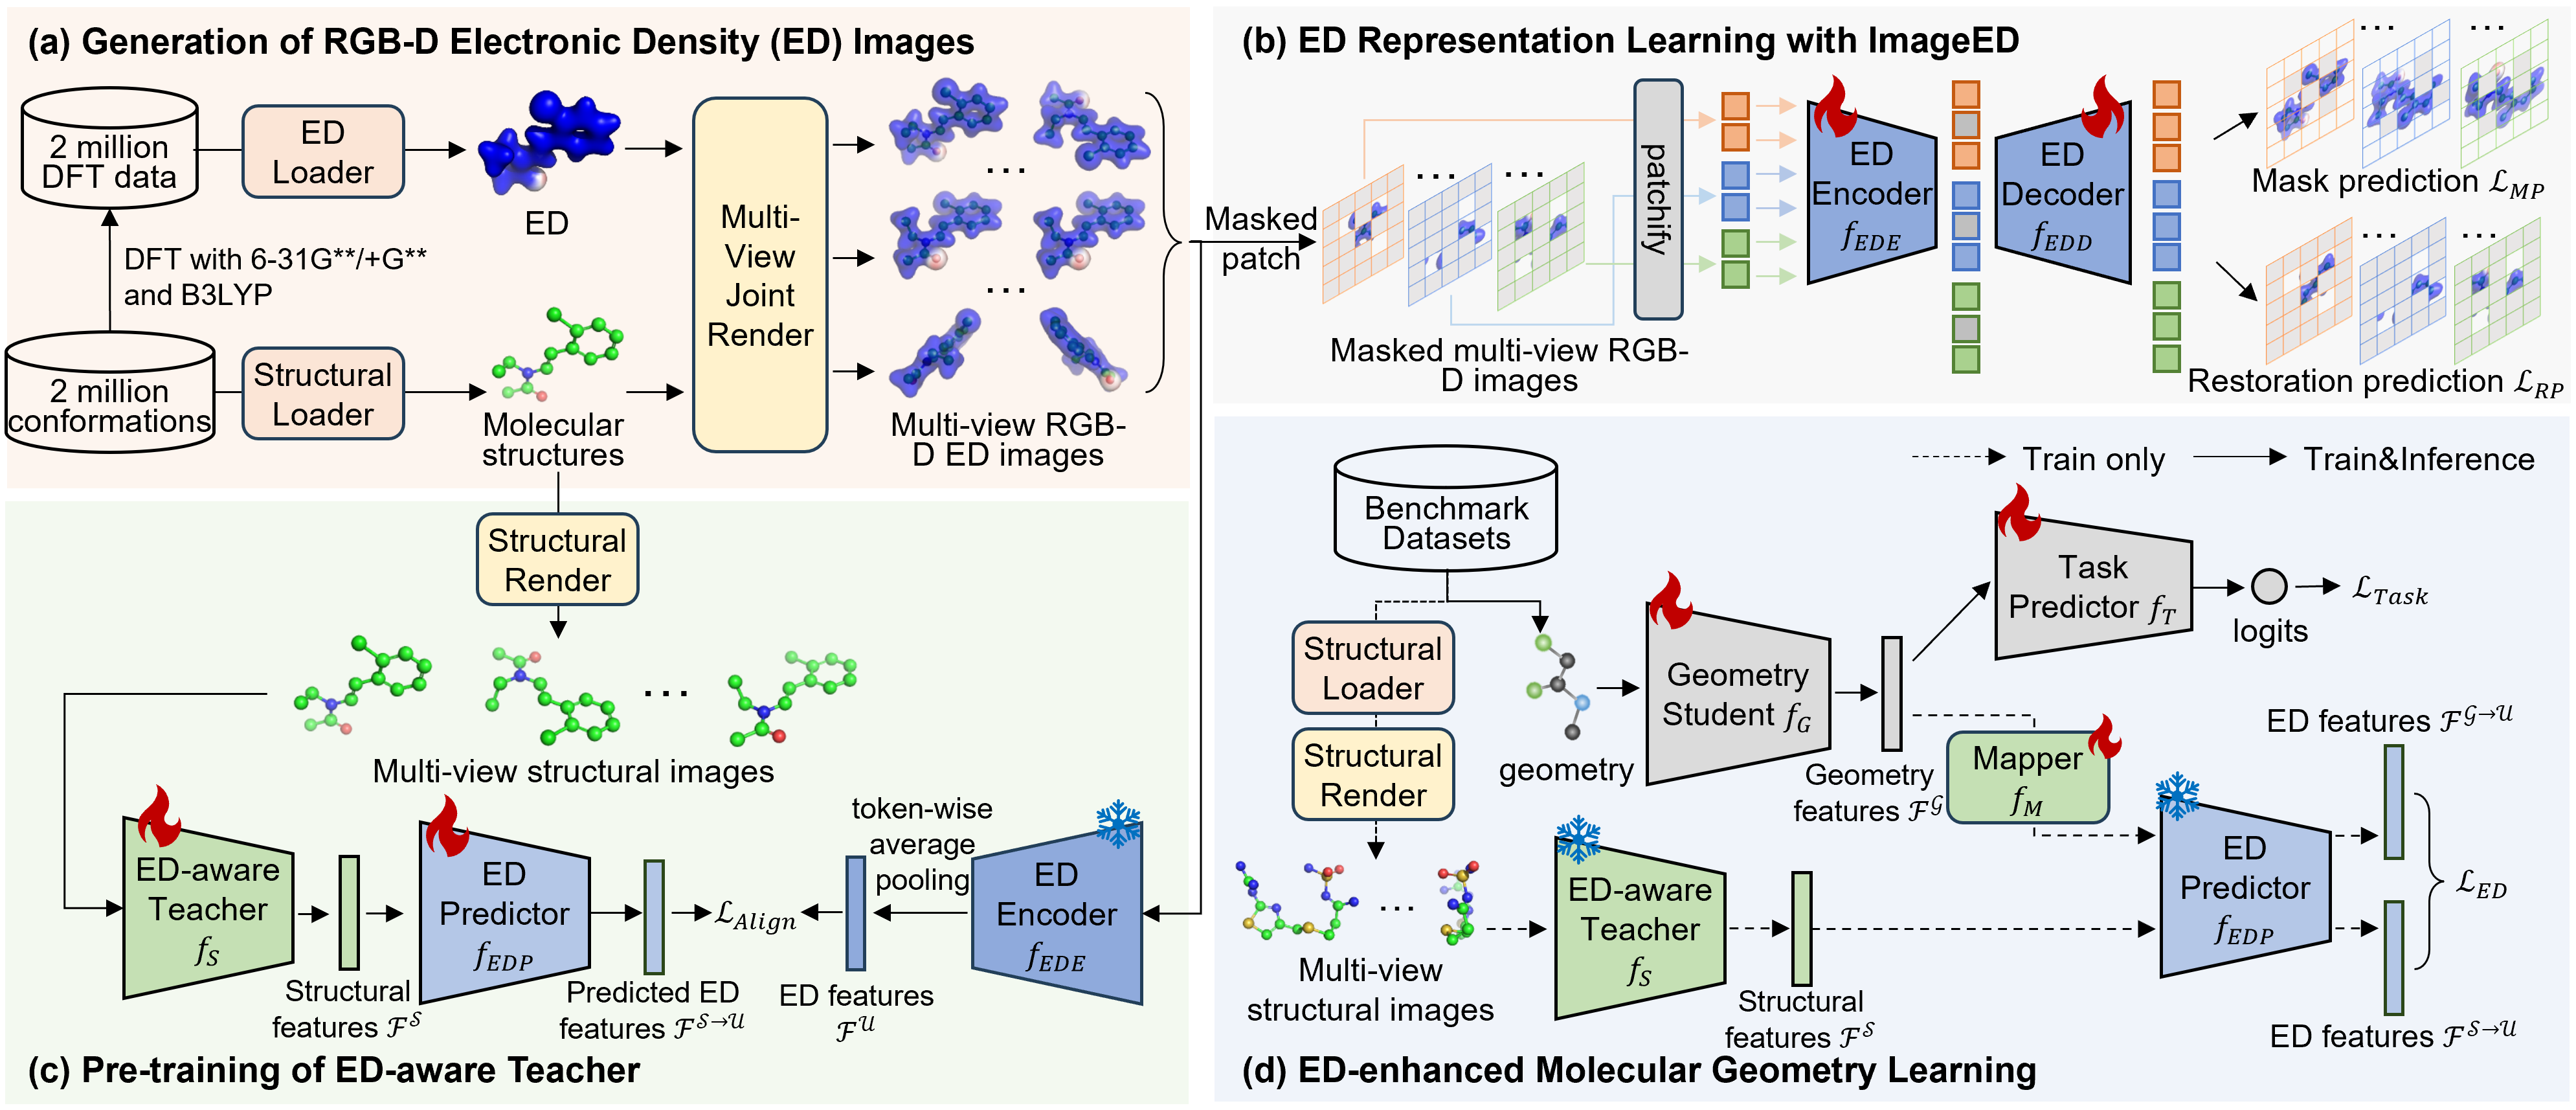
\includegraphics[width=16cm]{./imgs/our_method/EDG.png}
\caption{Overview of the proposed EDG framework. \textbf{(a)} Multi-view ED images with RGB-D channels are generated based on 2 million molecular conformers and DFT data, which contains the structural and ED information of the molecule. \textbf{(b)} ImageED with masked autoencoder (MAE) architecture and 2 pretext tasks ($\mathcal{L}_{MP}$ and $\mathcal{L}_{RP}$) is pretrained to extract ED-related features from multi-view ED images in (a). \textbf{(c)} The ED-aware teacher accepts the structural images as input and learns to transform it into ED features $\mathcal{F}^{\mathcal{S}\rightarrow\mathcal{U}}$ using ED predictor and ED encoder in (b). \textbf{(d)} In downstream tasks, the ED-aware teacher and ED predictor from (c) are frozen to enhance the geometry student. Note that there is no need for explicit involvement of electron density here because the ED teacher has the ability to extract ED-related information.}
\label{Fig2_Method}
\end{figure*}

\subsection{Generation of RGB-D Electron Density Images}
\label{sec:Generation_ED_Image}

As shown in Figure \ref{Fig2_Method}(a), we first obtain 2 million molecular conformations from PCQM4Mv2 \cite{hu2021ogb} and use density functional theory (DFT) with the basis set of 6-31G**/+G** and the exchange-correlation functional of B3LYP to generate DFT data for these molecular conformations \cite{sud2016mayachemtools}. For each molecule, the DFT data includes an electrostatic potential (ESP) file and an ED file stored in the form of a three-dimensional grid. Next, we describe the main details of ED image generation. The structural loader uses the command \textit{load \{conformation file\}} in PyMol \cite{delano2002pymol} to load the structural information from the molecular conformation file. ED loader uses the commands \textit{load \{ED file\}, ED; load \{ESP file\}, ESP; ramp\_new legend, ESP, [-0.08, 0, 0.08], [red, white, blue]; isosurface surface, ED, 0.05; set surface\_color, legend, surface} in PyMol to load the ED information, which uses a red-white-blue distribution range to describe the electrostatic potential distribution of ED and red, white, and blue represent positive, neutral, and negative regions, respectively. Finally, multi-view joint render uses commands \textit{set transparency, 0.4; turn \{axis\}, \{angle\}; png \{path\}, width=\{width\}, height=\{height\}} in PyMol to render the ED information and structural information into multi-view RGB-D ED images $\mathcal{U}\in\mathbb{R}^{6\times 4\times 224\times 224}$. Specifically, $\{axis\}$ and $\{angle\}$ represent the rotation angle degrees along axis and we set ($\{axis\}, \{angle\}$) to $(x, 0), (x, 180), (x, 90), (x, -90), (y, 90), (y, -90)$, which means generating images from 6 different views. $\{width\}=224$ and $\{height\}=224$ represent the width and height of the rendered image and $\{path\}$ represents the path where the image is saved. We describe more details of ED image rendering in Appendix E.


\subsection{ED Representation Learning with ImageED}
\label{sec:ED_representation_learning}

The proposed ED images have two properties: (1) RGB and D channels use color to represent the distribution of ED and depth to represent the spatial layout, respectively, which indicates that each pixel has a clear physical meaning; (2) the distribution of ED is continuous, which means that ED can be predicted by the context. Therefore, we propose a novel ED representation learning framework (called ImageED) with mask prediction and restoration prediction tasks to learn pixel-level local and contextual ED information from 2 million ED images. ImageED is an encoder-decoder architecture, which is built following the ViT-Large/16 \cite{dosovitskiy2020image} of MAE \cite{he2022masked}. For a given batch ($n$ molecules) of ED images $u\in\mathbb{R}^{n\times c\times V\times H\times W}$ (where $V, c, H, W=6, 4, 224, 224$), we first use a view-agnostic patch embed layer with a patch size of $n_p=16$ to transform $u$ into a pile of multi-view tokens $mt$. 
\begin{align}
\label{Formula_mt}
mt_{i,j}=u[:, :, n_p i: n_p (i+1), n_p j: n_p (j+1)]
\end{align}

We assume $n_t=H/n_p=W/n_p$ and $mt=\{mt_{i,j}|i, j\in\{0,1,...,n_t\}\}\in\mathbb{R}^{n\times V\times n_t^2\times (n_p^2\times c)}$. Next, we add the positional embeddings and expand along the view to get tokens $t=\in\mathbb{R}^{n\times (V\times n_t^2)\times (n_p^2\times c)}$. We shuffle the order of tokens and randomly mask 75\% of the tokens to obtain the masked tokens $t^m\in\mathbb{R}^{n\times(0.75\times V\times n_t^2)\times (n_p^2\times c)}$ and unmasked tokens $t^u\in\mathbb{R}^{n\times(0.25\times V\times n_t^2)\times (n_p^2\times c)}$ respectively. We input the $t^u$ into the ED encoder $f_{EDE}$ to get the encoded tokens: 
\begin{align}
\label{Formula_h_u}
h^u=f_{EDE}(t^u), h^u\in\mathbb{R}^{n\times(0.25\times V\times n_t^2)\times d_{\mathcal{U}}}
\end{align}
where $d_{\mathcal{U}}$ represents the feature dimension of $h^u$. Afterwards, we use additional mask tokens $\hat{h}^{m}$ that is initialized by 0 to the encoded tokens to obtain all encoded tokens $h$:
\begin{align}
\label{Formula_h}
h=\pi(h^u\parallel\hat{h}^{m})+pos\in\mathbb{R}^{n\times(V\times n_t^2)\times (n_p^2\times c)}
\end{align}
where $\pi$ represents arrange them in the order of the images and $pos$ represents the positional embeddings. The final predicted masked tokens $\hat{t}^m$ and unmasked tokens $\hat{t}^u$ can be obtained by input $h$ into the ED Decoder $f_{EDD}$. 

In order to optimize the $f_{EDE}$ and $f_{EDD}$ in ImageED, we define a mask prediction task $\mathcal{L}_{MP}$:
\begin{align}
\label{Formula_L_MP}
\mathcal{L}_{MP}=\frac{1}{n}\sum_{i=1}^n sim(t^u_i, \hat{t}^u_i)
\end{align}
where $sim()$ represents the Euclidean distance. However, we find that using only mask prediction tasks will limit the understanding of local features. We further introduce the restoration prediction task $\mathcal{L}_{RP}$:
\begin{align}
\label{Formula_L_RP}
\mathcal{L}_{RP}=\frac{1}{n}\sum_{i=1}^n sim(t^m_i, \hat{t}^m_i)
\end{align}

Finally, the overall loss function of ImageED is formulated:
\begin{align}
\label{Formula_L_ImageED}
\mathcal{L}_{ImageED}=\lambda_{MP}\mathcal{L}_{MP}+\lambda_{RP}\mathcal{L}_{RP}
\end{align}
where $\lambda_{MP}$ and $\lambda_{RP}$ is the balance coefficient and we set them to 1. After pre-training ImageED with 2 million molecules, we use the $f_{EDE}$ to extract ED features.


\subsection{Pretraining of ED-aware Teacher}
\label{sec:Pretraining_of_ED-aware_Teacher}

Since the generation of ED data requires a lot of computing resources, it is resource-intensive and impractical to calculate ED data for every downstream task. Therefore, we hope to use an easily accessible intermediary to replace ED to generate ED features. We assume that the molecular conformation, ED data generated by DFT, and ED features are $s, x, h$, respectively. The acquisition of ED features follows this path: $s\xrightarrow{\text{DFT}}x\xrightarrow{\text{ImageED}}h$, which shows that when $s$ is known, $x$ and $h$ can be obtained. Therefore, according to the probability chain rule, the joint probability distribution $p(h,x|s)$ can be decomposed into: $p(h,x|s)=p(h|x,s)\cdot p(x|s)$. According to the Markov hypothesis \cite{markov1960theory}, we can get: $p(h|x,s)=p(h|x)$. In order to simplify $p(h,x|s)$ to a probability distribution that is independent of $x$, we further marginalize $x$ (integrating with respect to $x$) and get:
\begin{align}
\label{Formula_p_h_s}
p(h|s)=\int p(h|x)\cdot p(x|s) dx
\end{align}

Therefore, we can approximate $p(h|x)\cdot p(x|s)$ by directly learning a $p(h|s)$. Here, we propose an ED-aware teacher $f_{\mathcal{S}}$ and ED predictor $f_{EDP}$ as $p(h|s)$ to learn the mapping of ED features directly from molecular conformations. We choose multi-view structural images as the input of the $f_{\mathcal{S}}$ (See Appendix F for specific reasons). Specifically, structural render uses command template \textit{turn \{axis\}, \{angle\}; png \{path\}} in PyMol to render molecular structures from 2 million conformations into multi-view images $\mathcal{S}$. Considering computational efficiency, we generate 4 views here and $(\{axis\}, \{angle\})$ is set to $(x, 0), (x, 180), (y, 180), (z, 180)$. $f_{\mathcal{S}}$ uses ResNet18 \cite{he2016deep} with a view-wise average pooling and $f_{EDP}$ is a Multilayer Perceptron (MLP) with Linear Layer$\rightarrow$Softplus Activator$\rightarrow$Linear Layer. Given a batch ($n$ molecules) of structural images $s$ from $\mathcal{S}$ and ED images $u$ from $\mathcal{U}$, we obtain structural features $\mathcal{F}^{\mathcal{S}}$ and ED features $\mathcal{F}^{\mathcal{S}\rightarrow\mathcal{U}}$:
\begin{align}
\label{Formula_F_S_U_and_F_S}
\mathcal{F}^{\mathcal{S}\rightarrow\mathcal{U}}=f_{EDP}(\mathcal{F}^{\mathcal{S}}); \mathcal{F}^{\mathcal{S}}=f_{\mathcal{S}}(s)
\end{align}

Next, we freeze the ED encoder that accepts ED images $u$ as input and use a token-wise average pooling to convert the token features output by the ED encoder into ED features $\mathcal{F}^{\mathcal{U}}$. Finally, we take $\mathcal{F}^{\mathcal{U}}$ as the ground-truth and train the ED-aware teacher and ED predictor to learn the mapping from structural features to ED features on 2 million molecules. The loss function $\mathcal{L}_{align}$ is defined as:
\begin{align}
\label{Formula_L_align}
\mathcal{L}_{align}=L1(\mathcal{F}^{\mathcal{S}\rightarrow\mathcal{U}}, \mathcal{F}^{\mathcal{U}})
\end{align}
where $L1$ represent L1 distance. With the ED-aware teacher, the costly ED image can be replaced by a cheaper structural image, significantly reducing DFT-related costs. %



\subsection{ED-enhanced Molecular Geometry Learning}
\label{sec:ED-enhanced_Molecular_Geometry_Learning}

In the training stage of downstream tasks, we first convert the molecular conformations in the dataset into geometric data and multi-view structural images using structural loader and structural render. Subsequently, geometry data and images are input into the geometry student $f_{G}$ and frozen ED-aware teacher to extract features $\mathcal{F}^{\mathcal{G}}$ and $\mathcal{F}^{\mathcal{S}}$, respectively. Please note that $f_{G}$ can be any geometry-based model, such as SchNet \cite{schutt2017schnet}, EGNN \cite{satorras2021n}, etc. Next, a mapper $f_M$ is used to map the geometry features into the structural space to obtain $f_M(\mathcal{F}^{\mathcal{G}})$. Subsequently, the frozen ED predictor accepts $f_M(\mathcal{F}^{\mathcal{G}})$ and $\mathcal{F}^{\mathcal{S}}$ as input and obtains predicted ED features:
\begin{align}
\label{Formula_L_align}
\mathcal{F}^{\mathcal{G}\rightarrow\mathcal{U}}=f_{EDP}(f_M(\mathcal{F}^{\mathcal{G}})); \mathcal{F}^{\mathcal{S}\rightarrow\mathcal{U}}=f_{EDP}(\mathcal{F}^{\mathcal{S}})
\end{align}

To distill the ED knowledge from the teacher model to the student model, we define a consistency loss $\mathcal{L}_{ED}$:
\begin{align}
\label{Formula_L_ED}
\mathcal{L}_{ED}=SL1(\mathcal{F}^{\mathcal{G}\rightarrow\mathcal{U}}, \mathcal{F}^{\mathcal{S}\rightarrow\mathcal{U}})
\end{align}
where $SL1$ represents smooth L1 distance \cite{girshick2015fast}. In order to obtain task-related labels, we define a task predictor $f_T$, which accepts geometry features $\mathcal{F}^{\mathcal{G}}$ to output task-related logits $\hat{y}=f_T(\mathcal{F}^{\mathcal{G}})$. The task-related loss function is defined as:
\begin{align}
\label{Formula_L_Task}
\mathcal{L}_{Task}=L1(\hat{y}, y)
\end{align}

The final loss of EDG is formulated:
\begin{align}
\label{Formula_L_ED}
L_{EDG}=\mathcal{L}_{Task}+\lambda\mathcal{L}_{ED},
\end{align}
where $\lambda$ is the balanced coefficient. In the inference phase, the prediction result is obtained by sequentially inputting the geometry data into the student network $f_G$ and the task predictor $f_T$. Therefore, images are only involved in the training of the model and are not needed during inference, which further improve the efficiency.






\section{Experiments and Results}

\subsection{Experimental Settings}
\textbf{Datasets and evaluation protocol.} To pre-train ImageED, the ED-aware teacher, and the ED predictor, we select the first 2 millions unlabeled molecular conformations and their DFT-computed ED data from the EDBench database \cite{xiang2025edbenchlargescaleelectrondensity}, generated by Psi4 software \cite{turney2012psi4} with a grid spacing of 0.4. In evaluation stage, we select 12 widely used tasks related to quantum mechanic properties from QM9 \cite{ramakrishnan2014quantum} and 10 common tasks related to energy/force from revised MD17 (rMD17) \cite{christensen2020role}. It is worth noting that for the force prediction, we first predict the molecular energy and use the gradient of each node position as the force, that is, \textit{force=-torch.autograd.grad(outputs=energy, inputs=positions)} in PyTorch \cite{paszke2019pytorch}. The dataset split follows Geom3D \cite{liu2024symmetry}, i.e., using 110K for training, 10K for validation, and 11K for testing in QM9 and 950 for training, 50 for validation, and 1000 for testing in rMD17. We use mean absolute error (MAE) as evaluation metric.

\textbf{Baselines.} To verify the effectiveness of EDG, we select many geometry-based models with different architectures, such as SchNet \cite{schutt2017schnet}, EGNN \cite{satorras2021n}, Equiformer \cite{liao2023equiformer}, SphereNet \cite{liu2022spherical}, ViSNet \cite{wang2024enhancing}, as geometry students to verify the generalizability of EDG. Following \cite{liu2022spherical,wang2024enhancing,liu2024symmetry}, we ensure that each baseline is fully trained. For example, SchNet, EGNN, and SphereNet are trained for 1,000 epochs with a learning rate of 5e-4; Equiformer is trained for 300 epochs with a learning rate of 5e-4; and ViSNet is trained for 3,000 epochs with a learning rate of 0.0002. The batch size of SchNet, EGNN, SphereNet, and Equiformer is set to 128 in QM9 and 1 in rMD17, the batch size of ViSNet is set to 4 in rMD17. 

\textbf{Implementation details.} The encoder and decoder of ImageED are built based on ViT-Large/16. In pre-training of ImageED on 2 million ED molecules, we use a learning rate of 1.5e-4, a batch size of 64, a mask ratio of 0.75, $\lambda_{MP}$ and $\lambda_{RP}$ of 1 for 20 epochs on 8 GeForce RTX 4090 (See Appendix G for more details). In pre-training of ED-aware teacher on 2 million molecules, we divide 2\% as validation set and the rest as training set. We use a learning rate of 5e-3 and a batch size of 128 to train the ED-aware teacher and ED predictor for about 280k steps (See Appendix H for more details). In distillation stage of EDG, we select hyper-parameters $\lambda$ from 1e-4 and 5e-4 to 1.0 with a 10x increasing in steps. Following \cite{wang2024enhancing,liu2024symmetry}, we run the experiments with exactly the same parameter settings as the baselines and report test scores corresponding to the best validation performance. The mapper and task predictor consists of a simple linear layer.

\subsection{Main Results}

\begin{table*}[h]
  \scriptsize
  \centering
    \begin{tabular}{ccccccccccccc}
    \toprule
        \multirow{2}{*}{Model} & $\alpha$ $\downarrow$ & $\nabla \mathcal{E}$ $\downarrow$ & $\mathcal{E}_\text{HOMO}$ $\downarrow$ & $\mathcal{E}_\text{LUMO}$ $\downarrow$ & $\mu$ $\downarrow$ & $C_v$ $\downarrow$ & $G$ $\downarrow$ & $H$ $\downarrow$ & $R^2$ $\downarrow$ & $U$ $\downarrow$ & $U_0$ $\downarrow$ & ZPVE $\downarrow$\\
        & $\alpha_0^3$ & $meV$ & $meV$ & $meV$ & $D$ & $\frac{cal}{mol\cdot K}$ & $meV$ & $meV$ & $\alpha_0^2$ & $meV$ & $meV$ & $meV$\\
    \midrule
    SchNet & 0.07021  & 50.829  & 31.952  & 26.168  & 0.03013  & 0.03228  & 14.678  & 14.090  & 0.13455  & 14.142  & 13.915  & 1.714  \\
    EDG-SchNet & 0.06866  & 49.778  & 31.884  & 25.972  & 0.02980  & 0.03162  & 14.022  & 13.841  & 0.12458  & 13.794  & 13.826  & 1.688  \\
    $\Delta$ & ↑2.2\% & ↑2.1\% & ↑0.2\% & ↑0.7\% & ↑1.1\% & ↑2.0\% & ↑4.5\% & ↑1.8\% & ↑7.4\% & ↑2.5\% & ↑0.6\% & ↑1.5\% \\
    \midrule
    EGNN  & 0.06474  & 49.493  & 29.865  & 24.696  & 0.02981  & 0.03125  & 11.057  & 10.596  & 0.07494  & 11.013  & 10.150  & 1.519  \\
    EDG-EGNN & 0.06147  & 46.979  & 28.319  & 24.283  & 0.02655  & 0.03078  & 10.708  & 10.298  & \textbf{0.07225}  & 9.985  & 10.012  & 1.498  \\
    $\Delta$ & ↑5.1\% & ↑5.1\% & ↑5.2\% & ↑1.7\% & ↑10.9\% & ↑1.5\% & ↑3.2\% & ↑2.8\% & ↑3.6\% & ↑9.3\% & ↑1.4\% & ↑1.4\% \\
    \midrule
    Equiformer & 0.06762  & 46.308  & 26.017  & 23.681  & 0.02074  & 0.02733  & 18.439  & 16.453  & 0.45828  & 15.339  & 23.928  & 1.537  \\
    EDG-Equiformer & 0.06476  & 45.813  & 25.492  & 23.266  & \textbf{0.01985}  & 0.02642  & 15.976  & 14.451  & 0.43947  & 15.466  & 16.517  & 1.529  \\
    $\Delta$ & ↑4.2\% & ↑1.1\% & ↑2.0\% & ↑1.8\% & ↑4.3\% & ↑3.3\% & ↑13.4\% & ↑12.2\% & ↑4.1\% & ↓0.8\% & ↑31.0\% & ↑0.5\% \\
    \midrule
    SphereNet & 0.04670  & 40.129  & 22.007  & 19.435  & 0.02689  & 0.02437  & 7.875  & 7.199  & 0.25821  & 6.999  & 6.641  & 1.253  \\
    EDG-SphereNet & \textbf{0.04592}  & \textbf{39.694}  & \textbf{21.842}  & \textbf{19.014}  & 0.02648  & \textbf{0.02376}  & \textbf{7.769}  & \textbf{6.283}  & 0.24935  & \textbf{6.502}  & \textbf{6.101}  & \textbf{1.206}  \\
    $\Delta$ & ↑1.7\% & ↑1.1\% & ↑0.7\% & ↑2.2\% & ↑1.5\% & ↑2.5\% & ↑1.3\% & ↑12.7\% & ↑3.4\% & ↑7.1\% & ↑8.1\% & ↑3.8\% \\
    \bottomrule
    \end{tabular}
  \caption{The mean absolute error (MAE) performance of different methods on 12 quantum mechanics prediction tasks in QM9. $\Delta$ represents the relative improvement percentage calculated by $(1-\frac{w/ EDG}{w/o EDG})\times 100$.}
  \label{tab:qm9}
\end{table*}


\begin{table*}[h]
  \scriptsize
  \centering
    \begin{tabular}{ccccccccccc}
    \toprule
    Model & Aspirin ↓ & Azobenzene ↓ & Benzene ↓ & Ethanol ↓ & Malona. ↓ & Naphth. ↓ & Paracetamol ↓ & Salicylic ↓ & Toluene ↓ & Uracil ↓ \\
    \midrule
    SchNet & 0.73909  & 0.39678  & 0.02052  & 0.12516  & 0.16142  & 0.21158  & 0.37097  & 0.19078  & 0.20797  & 0.07872  \\
    EDG-SchNet & 0.35525  & 0.33441  & 0.01711  & 0.06061  & 0.11181  & 0.07338  & 0.28303  & 0.15697  & 0.08780  & 0.07433  \\
    $\Delta$ & ↑51.9\% & ↑15.7\% & ↑16.6\% & ↑51.6\% & ↑30.7\% & ↑65.3\% & ↑23.7\% & ↑17.7\% & ↑57.8\% & ↑5.6\% \\
    \midrule
    SphereNet & 0.18091  & 0.09794  & 0.00647  & 0.03784  & 0.06005  & 0.03823  & 0.10425  & 0.14119  & 0.03452  & 0.08088  \\
    EDG-SphereNet & 0.13622  & 0.06788  & 0.00413  & 0.03575  & 0.05659  & 0.02753  & 0.09934  & 0.09569  & 0.02413  & 0.03683  \\
    $\Delta$ & ↑24.7\% & ↑30.7\% & ↑36.2\% & ↑5.5\% & ↑5.8\% & ↑28.0\% & ↑4.7\% & ↑32.2\% & ↑30.1\% & ↑54.5\% \\
    \midrule
    ViSNet & 0.05547  & 0.02081  & 0.00627  & 0.01095  & 0.01517  & 0.01313  & 0.02700  & 0.01966  & 0.01089  & 0.01238  \\
    EDG-ViSNet & \textbf{0.04650 } & \textbf{0.01838 } & \textbf{0.00616 } & \textbf{0.00990 } & \textbf{0.01395 } & \textbf{0.01178 } & \textbf{0.02491 } & \textbf{0.01906 } & \textbf{0.00998 } & \textbf{0.01188 } \\
    $\Delta$ & ↑16.2\% & ↑11.7\% & ↑1.8\% & ↑9.6\% & ↑8.0\% & ↑10.2\% & ↑7.8\% & ↑3.0\% & ↑8.3\% & ↑4.0\% \\
    \bottomrule
    \end{tabular}
  \caption{The MAE performance of different methods on 10 energy ($\frac{kcal}{mol}$) prediction tasks in rMD17. Malona. and Naphth. represents Malonaldehyde, Naphthalene, respectively. $\Delta$ represents the relative improvement percentage calculated by $(1-\frac{w/ EDG}{w/o EDG})\times 100$.}
  \label{tab:rmd17_energy}
\end{table*}


\begin{table*}[h]
  \scriptsize
  \centering
    \begin{tabular}{ccccccccccc}
    \toprule
    Model & Aspirin ↓ & Azobenzene ↓ & Benzene ↓ & Ethanol ↓ & Malona. ↓ & Naphth. ↓ & Paracetamol ↓ & Salicylic ↓ & Toluene ↓ & Uracil ↓ \\
    \midrule
    SchNet & 1.04245  & 0.90082  & 0.18569  & 0.38519  & 0.65536  & 0.39851  & 0.82544  & 0.77487  & 0.48322  & 0.51399  \\
    EDG-SchNet & 1.04910  & 0.91692  & 0.17113  & 0.37901  & 0.64678  & 0.39509  & 0.83296  & 0.74308  & 0.47790  & 0.50783  \\
    $\Delta$ & ↓0.6\% & ↓1.8\% & ↑7.8\% & ↑1.6\% & ↑1.3\% & ↑0.9\% & ↓0.9\% & ↑4.1\% & ↑1.1\% & ↑1.2\% \\
    \midrule
    SphereNet & 0.39134  & 0.21776  & 0.02151  & 0.19432  & 0.29278  & 0.11141  & 0.32265  & 0.28692  & 0.10978  & 0.27702  \\
    EDG-SphereNet & 0.38598  & 0.21665  & 0.02101  & 0.18741  & 0.28456  & 0.11102  & 0.32023  & 0.28299  & 0.10804  & 0.17179  \\
    $\Delta$ & ↑1.4\% & ↑0.5\% & ↑2.3\% & ↑3.6\% & ↑2.8\% & ↑0.3\% & ↑0.8\% & ↑1.4\% & ↑1.6\% & ↑38.0\% \\
    \midrule
    ViSNet & 0.15164  & 0.05729  & 0.00656  & 0.05688  & 0.09275  & 0.02808  & \textbf{0.10488 } & 0.08348  & 0.02980  & 0.05252  \\
    EDG-ViSNet & \textbf{0.14996 } & \textbf{0.05691 } & \textbf{0.00647 } & \textbf{0.05558 } & \textbf{0.08992 } & \textbf{0.02798 } & 0.10599  & \textbf{0.08107 } & \textbf{0.02780 } & \textbf{0.05100 } \\
    $\Delta$ & ↑1.1\% & ↑0.7\% & ↑1.3\% & ↑2.3\% & ↑3.0\% & ↑0.3\% & ↓1.1\% & ↑2.9\% & ↑6.7\% & ↑2.9\% \\
    \bottomrule
    \end{tabular}
  \caption{The MAE performance of different methods on 10 force ($\frac{kcal}{mol\cdot \text{\r{A}}}$) prediction tasks in rMD17. Malona. and Naphth. represents Malonaldehyde, Naphthalene, respectively. $\Delta$ represents the relative improvement percentage calculated by $(1-\frac{w/ EDG}{w/o EDG})\times 100$.}
  \label{tab:rmd17_force}
\end{table*}


We first evaluate the performance of EDG on the 12 quantum properties from QM9 with 4 baselines (SchNet, EGNN, Equiformer, SphereNet) and Table \ref{tab:qm9} shows the main results. We find baselines equipped with EDG achieve the best performance. We observe that regardless of the architecture, the baselines after equipping EDG achieve consistent performance improvement with a relative performance increase ranging from 2.2\% to 6.4\% in average MAE performance. Except for the property $U$ in Equiformer, all other performance are enhanced.

In order to verify the effectiveness of EDG in more tasks, we further evaluate on 10 energy/force prediction tasks from rMD17 with 3 baselines (SchNet, SphereNet, ViSNet). Table \ref{tab:rmd17_energy} and Table \ref{tab:rmd17_force} show the prediction performance on energy and force respectively. We find the same conclusion as on the QM9 benchmark, that is, EDG improves the performance of all baselines with average MAE performance improvements ranging from 8.1\% to 33.7\% on energy and 1.5\% to 5.3\% on force. It is worth noting that EDG has a larger improvement on energy prediction than on force. This is because ED can capture the global energy distribution, while force, as an energy gradient, depends on local atomic interactions, making the improvement brought by ED is not as obvious as energy. In any case, the performance improvements on energy and force prove the effectiveness of EDG. In addition, we also visualize absolute value of the difference between the predicted energy $y_{pred}$ and the ground-truth $y_{true}$ for all trajectories in the test set by showing the absolute value of the difference between them in Figure \ref{fig:rMD17_vis}, which shows that EDG outperforms the baselines in energy prediction for almost all trajectories.


\begin{figure}[!htb]
\centering
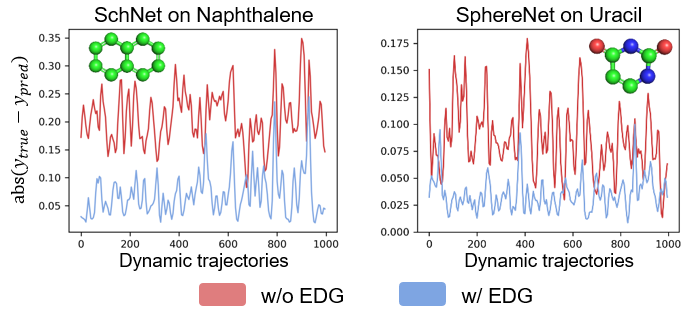
\includegraphics[width=8.5cm]{./imgs/experiments/rMD17_vis.png}
\caption{The visualization of SchNet on Naphthalene task and SphereNet on Uracil task. The $y$ axis represents the absolute value of the difference between $y_{pred}$ and $y_{true}$ on the test set.}  %
\label{fig:rMD17_vis}
\end{figure}


\subsection{Hyperparameters Analysis}

\begin{figure*}[!htb]
\centering
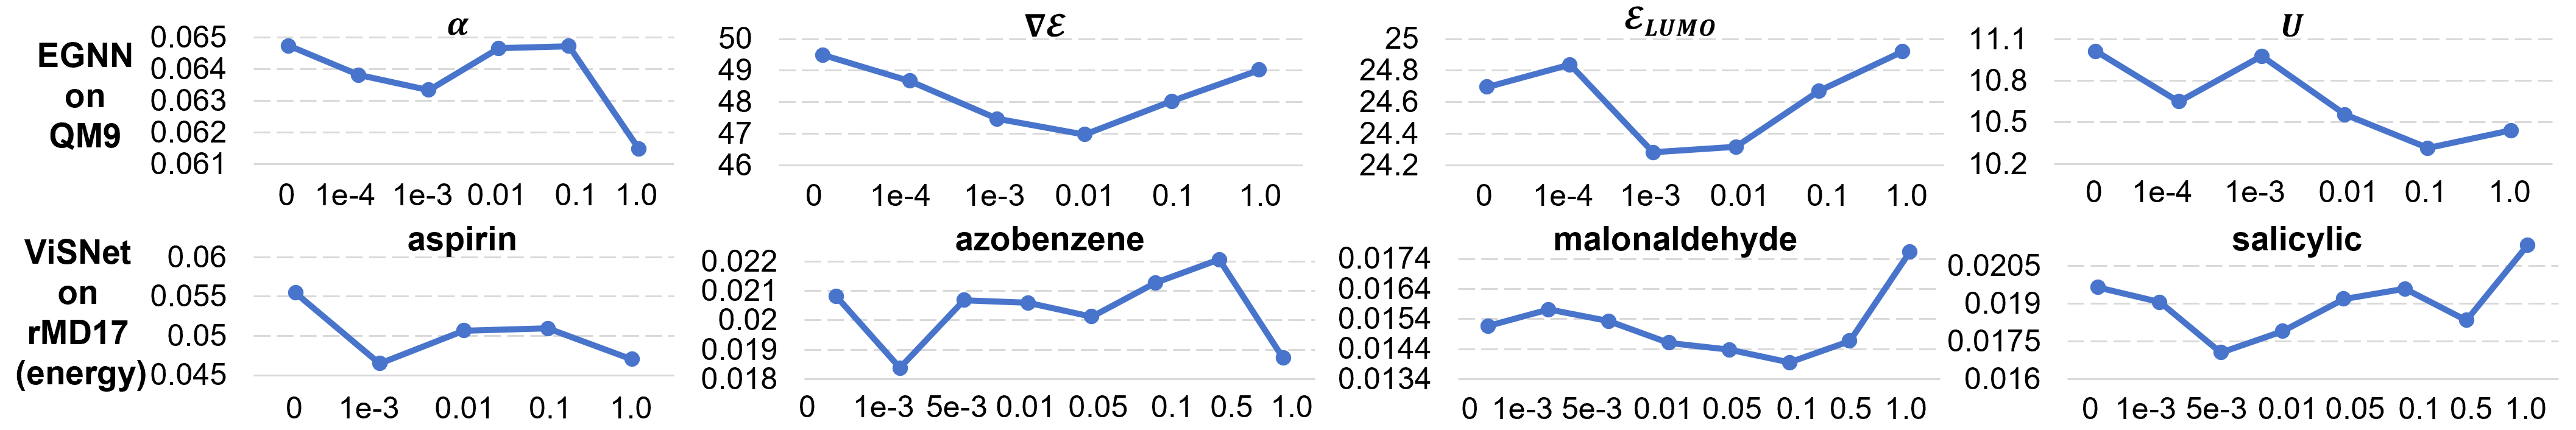
\includegraphics[width=17.8cm]{./imgs/experiments/lambda_ED.png}
\caption{Performance of EDG with different $\mathcal{L}_{ED}$. The $x$ axis and $y$ axis represent the value of $\mathcal{L}_{ED}$ and the corresponding MAE performance, respectively. $\mathcal{L}_{ED}=0$ means that EDG is not used.} %
\label{fig:lambda_ED}
\end{figure*}


$\lambda$ in Formula \ref{Formula_L_ED} is a parameter used to control the strength of distilling knowledge from the ED-aware teacher into the geometry students and a larger value will force the student to learn more knowledge from the teacher. Figure \ref{fig:lambda_ED} shows the line figures of the performance of EGNN and ViSNet with different $\mathcal{L}_{ED}$ on QM9 and rMD17, respectively. Overall, we find that EDG can improve the performance of baselines to varying degrees with $\mathcal{L}_{ED}$. For example, on the aspirin task, the performance gain of EDG fluctuates from 8.2\% to 16.2\% with the adjustment of $\mathcal{L}_{ED}$. In addition, we also find several patterns: on the $\alpha$ and $U$ tasks, as $\mathcal{L}_{ED}$ increases, the performance decreases overall; on the $\nabla \mathcal{E}$, $\mathcal{E}_\text{LUMO}$, aspirin, and malonaldehyde tasks, the performance curve changes with $\mathcal{L}_{ED}$ in a U-shaped manner. These findings suggest that by tuning the appropriate $\mathcal{L}_{ED}$, EDG can better enhance the baselines.




\subsection{Results of ED images on Energy-related Tasks}

Here, we describe the advantages of the proposed ED image on energy-related tasks. We sample 10,000 molecules from 2 million DFT data and predict the energy of the molecular system given the ED information. We use exactly the same experimental settings and hyperparameters and randomly split the dataset into training/validation/test sets with an 8:1:1 ratio for evaluation. More settings see Appendix B. For each ED representation, we select the corresponding popular encoder to extract features, such as point cloud-based PointNet \cite{qi2017pointnet}, voxel-based ResNet3D \cite{hara2018can} and image-based ResNet18 \cite{he2016deep}. As shown in Table \ref{tab:results_ED_images}, we find the proposed ED iamge achieves the best performance on 6 energy-related tasks with a relative performance gain ranging from 7.8\% to 71.6\%, which demonstrates the effectiveness of image as a representation of ED and that 2D images are easier to learn compared to 3D representations.


\begin{table}[htbp]
  \scriptsize
  \centering
    \begin{tabular}{ccccccc}
    \toprule
    Models & E1    & E2    & E3    & E4    & E5    & E6 \\
    \midrule
    Point & 275.1  & 168.6  & 557.7  & 244.8  & 14.5  & 288.9  \\
    Voxel & 121.1  & 313.9  & 947.8  & 271.2  & 7.9   & 202.0  \\
    Image & \textbf{111.6} & \textbf{47.9} & \textbf{349.8} & \textbf{85.6} & \textbf{4.4} & \textbf{124.5} \\
    \midrule
    $\Delta$ & ↑7.8\% & ↑71.6\% & ↑37.3\% & ↑65.0\% & ↑44.5\% & ↑38.4\% \\
    \bottomrule
    \end{tabular}
   \caption{RMSE (Root Mean Squared Error) performance of different ED representations on 6 energy prediction tasks. Point (point cloud), voxel, and image use PointNet, ResNet3D, and ResNet18 as encoders, respectively. E1-E6 represent DF-RKS Final Energy, Nuclear Repulsion Energy, One-Electron Energy, Two-Electron Energy, DFT Exchange-Correlation Energy, and Total Energy, respectively. $\Delta$ represents the relative performance gain of the image compared to the best other results.}
  \label{tab:results_ED_images}
\end{table}


\subsection{Visualization of ImageED}

As shown in Figure \ref{fig:vis_ImageED}, we find that ImageED can generate ED images well compared original images, which indicates that ImageED can learn ED-related knowledge well. In addition, we find that simply applying the masked prediction task (ImageED w/o $\mathcal{L}_{RP}$) will limit the understanding of ImageED in local pixels, which shows the importance of restoration prediction task in ImageED. We show more examples in the Appendix I.

\begin{figure}[!htb]
\centering
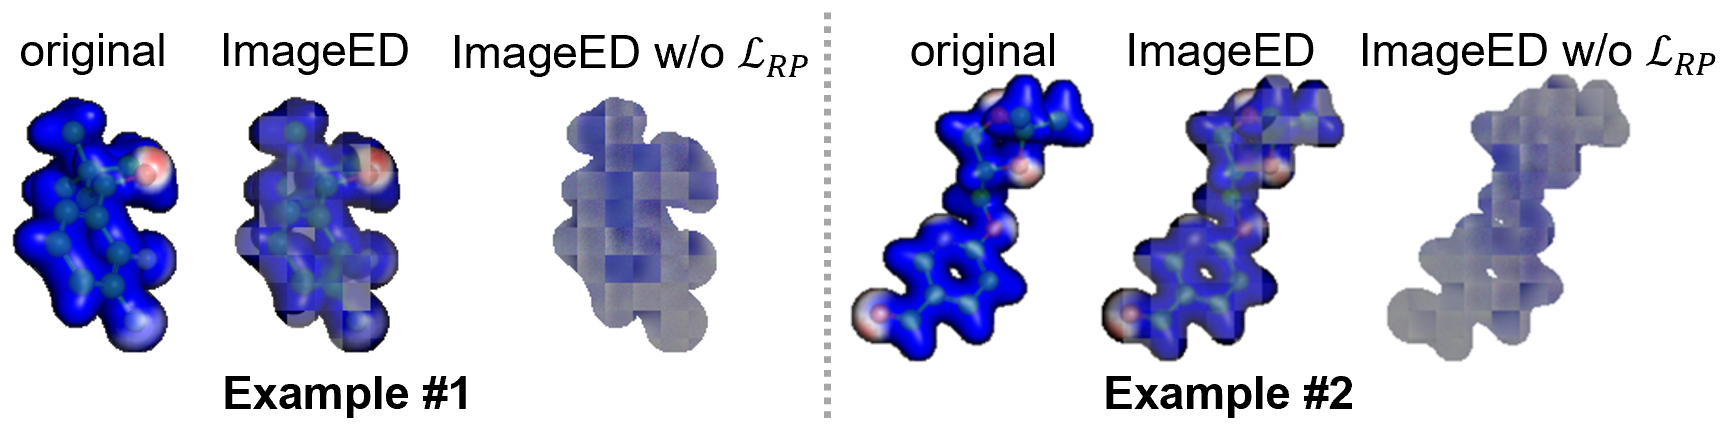
\includegraphics[width=8.5cm]{./imgs/experiments/ImageED_output.png}
\caption{Several examples of ImageED output visualizations.}
\label{fig:vis_ImageED}
\end{figure}





\section{Conclusion}
\label{Conclusion}

In this work, we propose a novel \textbf{ED}-enhanced molecular \textbf{G}eometry representation learning framework (called EDG), which is the first attempt to exploit ED images to improve the performance of geometry-based methods. We propose an efficient ED representation learning, called ImageED, to extract ED knowledge from images and further transfer the knowledge in ImageED to an ED-aware teacher to save the cost of DFT. By exploiting ED-aware teacher, EDG can significantly improve the performance of geometry-based methods without any architectural modifications on a large number of quantum chemical benchmarks. In addition, we experimentally show that using ED images can more accurately predict energy-related prediction tasks while saving memory and computational costs, enabling direct use of ED images in broader tasks like drug discovery and materials science. %



\section*{Acknowledgments}
This work was supported by the National Natural Science Foundation of China (grant nos. U22A2037, 62425204, 62122025, 62450002, 62432011), Grants of Ningbo 2023CX050011. %































































































































\bibliographystyle{named}
\bibliography{ijcai25}

\end{document}
